% id: 98-184
% book: 개념원리 기하 · 12 이면각
% section: 필수·발전 예제
% figure: crop:fig-98-184.png
% answer: $\dfrac{\sqrt{6}}{3}$
% answer_source: 답지
% variant_level: 0 (원본 전사)
% 이 파일은 build.mjs 가 items.json 에서 만든다. 고칠 때는 items.json 을 고친다.
\smash{\raisebox{1.5mm}{\dmkichul{개념원리 기하 98쪽 184번 · 확인체크}}}
\noindent\begin{minipage}[t]{0.58\linewidth}\vspace{0pt}\raggedright 오른쪽 그림과 같은 정사면체에서 $\seg{AD}$의 중점을 $\pt{M}$이라 하고, 평면~$\pt{ABC}$와 평면~$\pt{MBC}$가 이루는 각의 크기를 $\theta$라 할 때, $\cos\theta$의 값을 구하시오.\end{minipage}\hfill\begin{minipage}[t]{0.4\linewidth}\vspace{0pt}\centering \setlength{\dmfigw}{79.8pt}\ifdim\dmfigw>\linewidth\setlength{\dmfigw}{\linewidth}\fi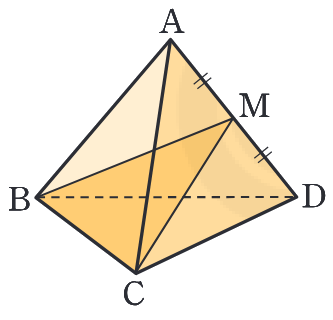
\includegraphics[width=\dmfigw]{figures/fig-98-184.png}\end{minipage}\par
